\chapter{Conclusión y líneas futuras}\label{chapter5}

Una vez expuestos todos los resultados de los capítulos anteriores, podemos concluir que hemos cumplido todos los objetivos propuestos en la introducción de este trabajo, además de haber realizado varios logros clave:
\begin{enumerate}
    \item Estudio de los \textbf{algoritmos de rasterización y \textit{raytracing}} de visualización por computador, y cómo combinarlos para el renderizado de superficies definidas por SDFs de forma eficiente en la gran mayoría de dispositivos actuales usando técnicas de iluminación avanzadas y \textit{antialiasing}, elaborando los \textit{vertex} y \textit{fragment shaders} necesarios.
    \item Implementación de una \textbf{librería de código abierto propia en TypeScript} para el manejo de polinomios en varias variables, incluyendo implementaciones de algoritmos de cálculo de bases de Gröbner e implicitación.
    \item Desarrollo de una \textbf{aplicación web con React eficiente, accesible a todo el mundo, y de código abierto}, que permite definir y modificar con una gran variedad de operadores superficies definidas mediante SDFs y ecuaciones paramétricas o implícitas.
\end{enumerate}
En el transcurso de la obtención de estos resultados ha sido necesario hacer una intensiva labor de investigación a través de artículos y documentaciones del ámbito tanto matemático como informático. Además, para asegurar la calidad y buen funcionamiento de los productos \textit{software} elaborados, tanto de la aplicación como de la librería, se han realizado pruebas de rendimiento y tests de forma constante durante su desarrollo.\newline

Considero que el \textit{software} desarrollado en este trabajo realiza una valiosa \textbf{contribución} al panorama actual. La librería de polinomios es la única que existe a fecha de realización de este trabajo para trabajar con polinomios en varias variables y bases de Gröbner de forma nativa en TypeScript. De forma similar ocurre con la aplicación web. Si bien existen aplicaciones web que permiten manipular SDFs como se mencionó al principio del documento, ninguna implementa el modelo de árbol ni permite que el usuario defina nuevas primitivas a partir de SDFs, y mucho menos que introduzca  sus ecuaciones paramétricas o implícitas.\newline

Entre las \textbf{futuras líneas} de desarrollo de la aplicación es de especial interés añadir la posibilidad de trabajar con mallas de polígonos. Existen métodos tanto para obtener una SDF aproximada dada una malla de triángulos \cite{meshToSDF2, meshToSDF3, meshToSDF4, meshToSDF5}, como para obtener una malla a partir de una SDF \cite{sdfToMesh, sdfToMesh2, sdfToMesh3, sdfToMesh4}. La inclusión de esta funcionalidad (\autoref{fig:meshToSDF}) añadiría una función muy interesante a la aplicación que hemos desarrollado, y permitiría un flujo de trabajo mucho más cómodo entre ella y programas de edición y visualización de geometría de terceros, pues trabajar con mallas sigue siendo lo más común en la industria actual. 
\begin{figure}[!ht]
    \centering
    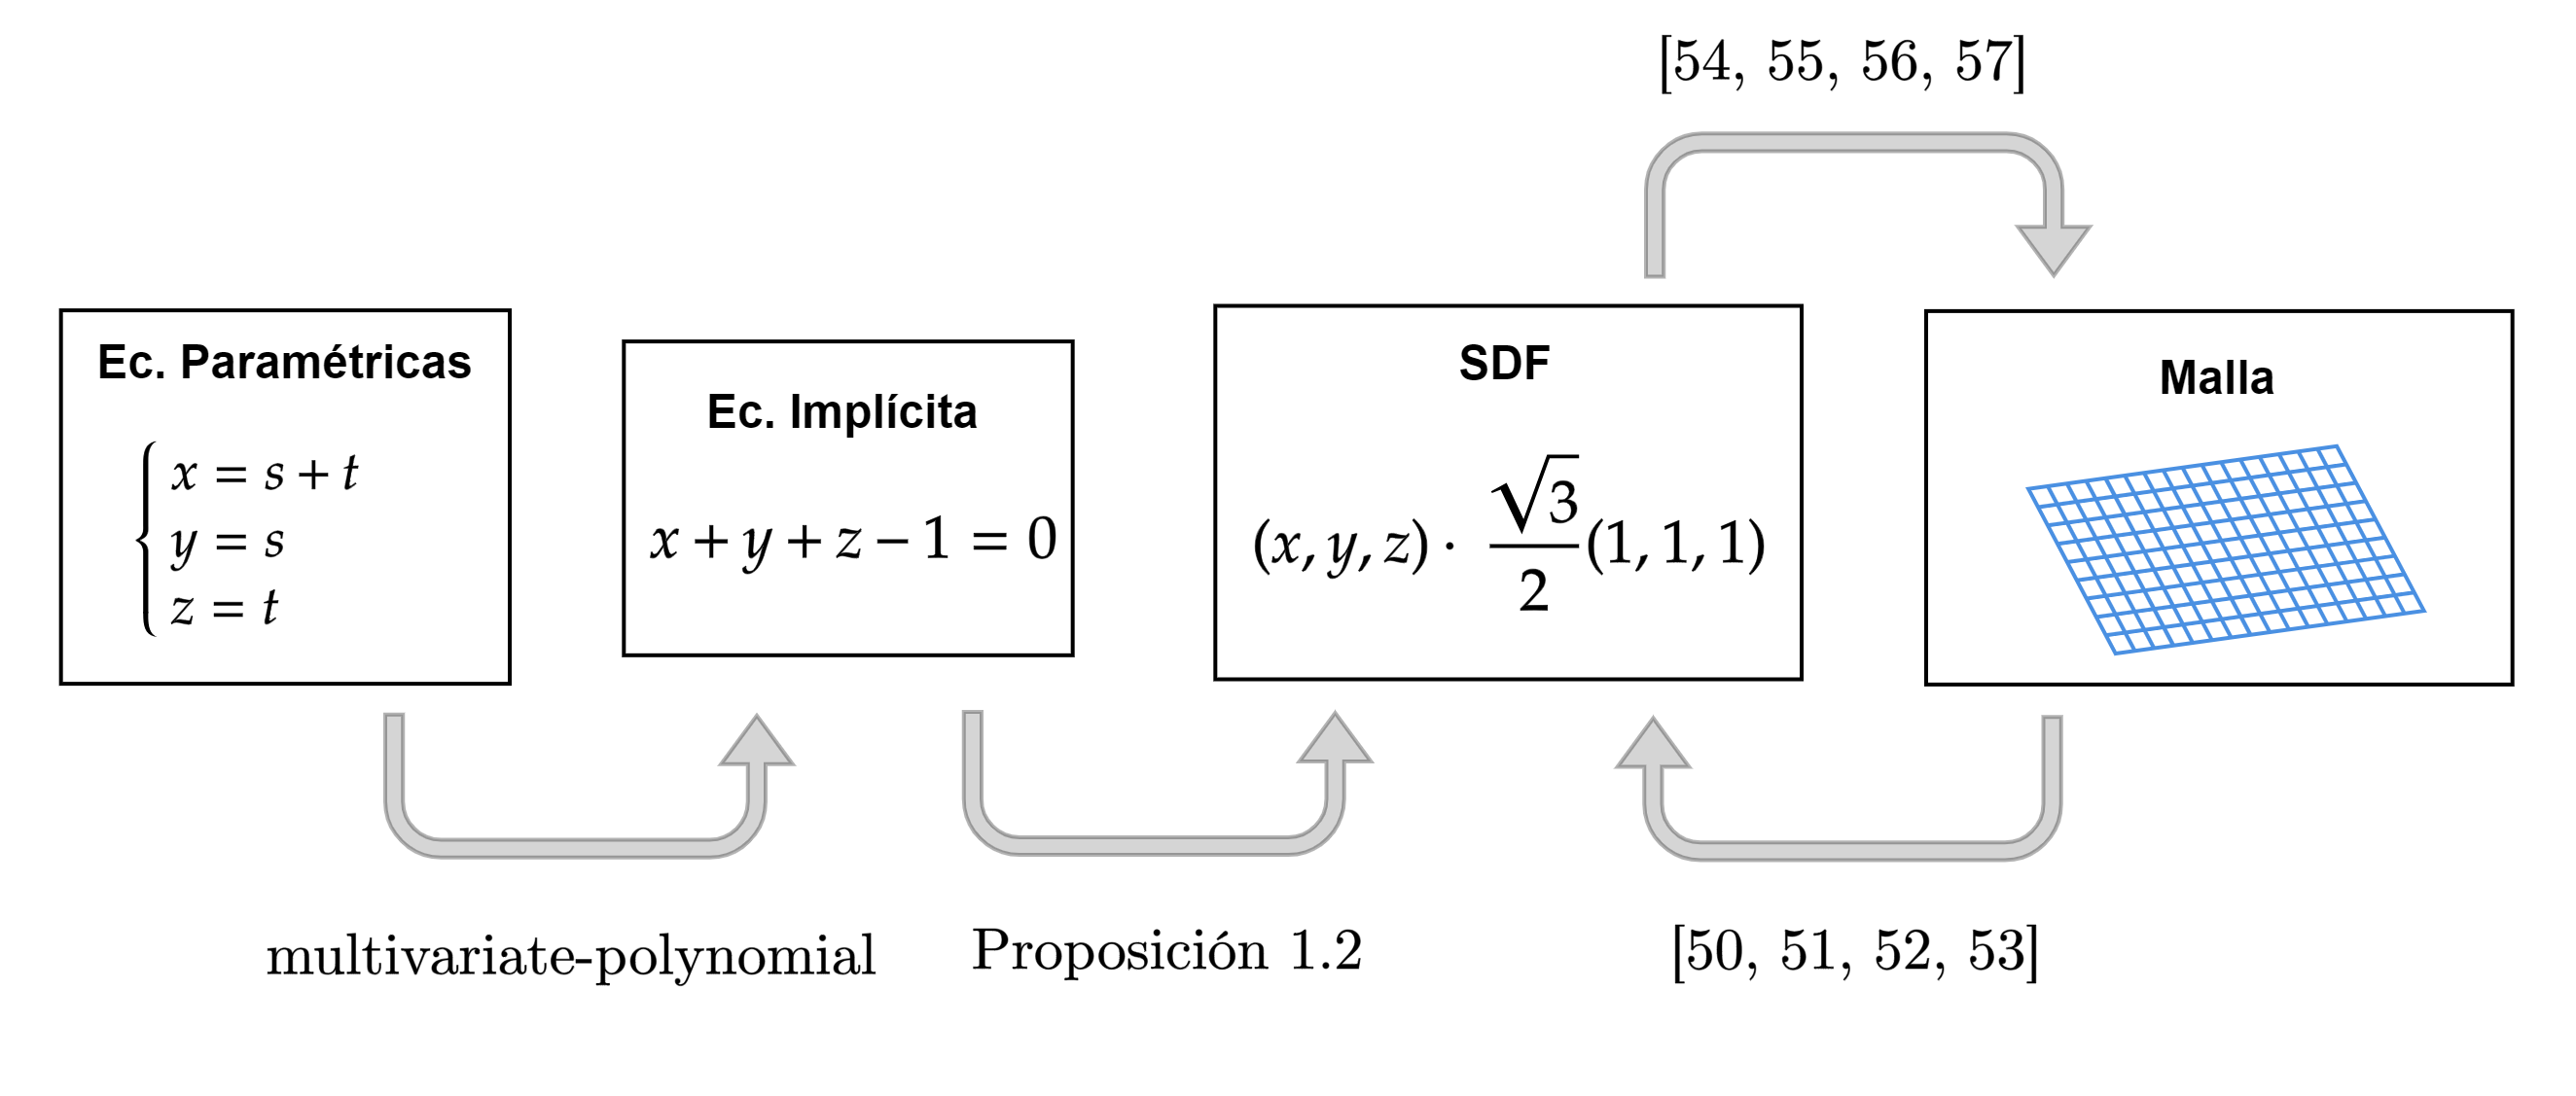
\includegraphics[width=\textwidth]{Plantilla-TFG-master/img/meshToSDF.png}
    \caption{Inclusión de compatibilidad con mallas de polígonos}
    \label{fig:meshToSDF}
\end{figure}
Otras posibilidades de mejora más sencillas para la aplicación son las relacionadas con la extensión de formas de manipulación de las superficies definidas por SDFs, tales como añadir la posibilidad de trabajar con texturas o la definición de materiales procedurales, o pulir ciertos aspectos de compatibilidad en dispositivos móviles, en los que si bien la aplicación es funcional, la interfaz o la visualización de superficies presenta defectos en algunos modelos.\newline

La librería \texttt{multivariate-polynomial} tiene también margen de mejora, siendo de especial interés permitir usar otros órdenes admisibles que no sean \textit{lex}, como \textit{degrevlex} o cualquier otro que defina el usuario. Quedan también versiones y mejoras del algoritmo de Buchberger por investigar \cite{conc1,conc2,conc3,conc4}. Es cierto que muchas de ellas serían poco prácticas en el entorno de una aplicación web \cite{conc5}, pero podrían suponer una mejora muy interesante para el uso de la librería en otros ámbitos. Ambos cambios mencionados se verían también reflejados en el rendimiento de la aplicación, pues el orden elegido influye en el número de reducciones a cero realizadas en el algoritmo de Buchberger, y este representa la mayor parte del tiempo de ejecución del algoritmo de implicitación racional. También merece la pena explorar algoritmos alternativos para el cálculo de bases de Gröbner, como es el $F_4$ o el $F_5$ \cite{conc6, conc7}. Por último, otra vía interesante es expandir la funcionalidad de la clase \texttt{Ideal} más allá de su uso para realizar implicitación, añadiendo nuevas operaciones, como la suma, división o saturación de ideales, y métodos que comprueben ciertas propiedades del ideal, como si es primario, su dimensión o la pertenencia de un polinomio a su radical, etc.